\documentclass[12pt,a4paper,english]{article}
\usepackage{times}
\usepackage[utf8]{inputenc}
\usepackage{babel,textcomp}
\usepackage{mathpazo}
\usepackage{mathtools}
\usepackage{amsmath,amssymb}
\usepackage{ dsfont }
\usepackage{listings}
\usepackage{graphicx}
\usepackage{ mathrsfs }
\usepackage{float}
\usepackage{subfig} 
\usepackage{multirow}
\usepackage[hyphens]{url}
\usepackage[colorlinks]{hyperref}
\hypersetup{breaklinks=true}
\usepackage[usenames,dvipsnames,svgnames,table]{xcolor}
\usepackage{textcomp}
\definecolor{listinggray}{gray}{0.9}
\definecolor{lbcolor}{rgb}{0.9,0.9,0.9}
\lstset{backgroundcolor=\color{lbcolor},tabsize=4,rulecolor=,language=python,basicstyle=\scriptsize,upquote=true,aboveskip={1.5\baselineskip},columns=fixed,numbers=left,showstringspaces=false,extendedchars=true,breaklines=true,
prebreak=\raisebox{0ex}[0ex][0ex]{\ensuremath{\hookleftarrow}},frame=single,showtabs=false,showspaces=false,showstringspaces=false,identifierstyle=\ttfamily,keywordstyle=\color[rgb]{0,0,1},commentstyle=\color[rgb]{0.133,0.545,0.133},stringstyle=\color[rgb]{0.627,0.126,0.941},literate={å}{{\r a}}1 {Å}{{\r A}}1 {ø}{{\o}}1}

% Use for references
\usepackage[square,comma,numbers]{natbib}
%\DeclareRobustCommand{\citeext}[1]{\citeauthor{#1}~\cite{#1}}

% Fix spacing in tables and figures
%\usepackage[belowskip=-8pt,aboveskip=5pt]{caption}
%\setlength{\intextsep}{10pt plus 2pt minus 2pt}

% Change the page layout
%\usepackage[showframe]{geometry}
%\usepackage{layout}
\setlength{\hoffset}{-0.7in}  % Length left
\setlength{\voffset}{-0.8in}  % Length on top
\setlength{\textwidth}{480pt}  % Width /597pt
\setlength{\textheight}{675pt}  % Height /845pt
%\setlength{\footskip}{25pt}

\newcommand{\VEV}[1]{\langle#1\rangle}
\title{FYS4411 - Project 2\\ The restricted Boltzmann machine applied to the quantum many-body problem}
\date{}
\author{ Kristoffer Langstad \footnote{\url{https://github.com/krilangs/FYS4411/tree/master/Project2} \cite{GitHub}}\\ \textit{krilangs@uio.no}}

\begin{document}%\layout
\maketitle
\begin{abstract}
In this project we study fermions in a harmonic oscillator potential using a restricted Boltzmann machine (RBM) to approximate the wave function as a neural network quantum state (NQS) combined with a variational Monte Carlo (VMC) method. To compute the ground state of the system, a stochastic gradient descent (SGD) method is used, and to do a statistical analysis of the results we use blocking. The computation of the system is tested with three sampling methods; a standard brute-force Metropolis method, Importance sampling and Gibbs sampling.

The computed energies in atomic units (a.u.) are benchmarked against analytical ground state energies for systems of one and two electrons in one and two dimensions with and without interaction. The computed results are found to have a strong dependence on the initial guesses of the variational/RBM parameters of the system, together with the sampling and learning rate parameters. For both the non-interacting and interacting cases the Gibbs method is found to give the best solutions and on average the best errors with the found optimal parameters, but all three sampling methods produce good energies close to the expected analytical energies. 
\end{abstract}


\section{Introduction}
\label{sect:Introduction}
Machine learning is a more and more used method in physics to simulate and study quantum systems. One of the categorizations in machine learning where we consider the desired output of a system, is Neural Networks (NN) and Boltzmann machines. Boltzmann machines are a type of unsupervised learning method. One application is to represent a wave function with a restricted Boltzmann machine (RBM). Such a wave function/network is named a neural network quantum state (NQS) after \citet{carleo2017solving}, which used this on quantum mechanical spin lattice systems of the Ising model and Heisenberg mode.

In this project we will test the applicability of the RBM's to quantum mechanics on a system with electrons confined to move in a harmonic oscillator trap. The system will be studied in one and two dimensions for one and two particles with different number of hidden nodes for non-interacting particles. Here, we can derive the ground state energy analytically. For the interacting case we only study two electrons in a quantum dot in two dimensions with various number of hidden nodes. In this case, we will compare our computed energies with analytical ground state energies from \citet{taut1993two}.

To do the ground state energy calculation, we will use Variational Monte Carlo (VMC) methods with three different sampling methods: a standard "brute-force" Metropolis sampling, an improved Metropolis-Hastings/Importance sampling and Gibbs sampling. We will use a Gaussian-Binary RBM as the neural networks (NN) with visible and hidden nodes to represent the wave function. The weights of these nodes are what we will use as variational parameters to approximate the ground state. We also use a Stochastic Gradient Descent (SGD) with a fixed learning rate to find the parameters that minimize the energy function. Then we do a statistical error analysis on the ground state energies by using the blocking method.

For the layout of this project, we first take a look at the theory of the physics and the numerics we will use in this project. Here get an overview of the physical system, neural networks, restricted Boltzmann machine, the analytical derivations of the ground state energies and then the theory of the numerical methods we are using. In the methods section, we explain what we do with the implementation of the numerical tools we use and the parameters we use for running the code. Here we will use the three sampling methods we have mentioned to sample the ground state energies for varying parameters and various cases. The computed energies, with a statistical analysis, will be benchmarked against the analytically derived ground state energies to see how well our sampling methods can compare with the analytical results. In the results section, we present and discuss the results we get from the VMC computation. Lastly, we come up with a conclusion to the project with possible aspects towards future work.


\section{Theory}
\label{sect:Theory}
\subsection{The System}
\label{subsect:System}
We will consider a system of $N_p=2$ electrons as function of the oscillator frequency $\omega$, confined in a pure 2D isotropic harmonic oscillator. With two electrons we can exclude Pauli's exclusion principle, which states that no more than two fermions can occupy the same quantum state simultaneously, and the Slater determinant. This system is considered as a quantum dot with frequency $\hbar\omega=1$. For this system we have exact closed form expressions for the ground state energy from \citet{taut1993two} for selected values for $\omega$ to use as benchmarks. The total Hamiltonian, with natural units ($\hbar=c=e=m_e=1$), of this system is given as 
\begin{equation}
\label{eq:Hamlitonian}
\hat{H}=\hat{H}_0+\hat{H}_1=\sum_{i=1}^{N_p}\left(-\frac{1}{2}\nabla^2_i + \frac{1}{2}\omega^2r_i^2\right) + \sum_{i<j}\frac{1}{r_{ij}}.
\end{equation}
Here $\hat{H}_0$ is the standard harmonic oscillator part, which is the Hamiltonian we will use without interaction between the electrons, and $\hat{H}_1$ is the repulsive interaction given by the Coulomb potential. The energies are in atomic units (a.u.), while the modulus of the position for an electron $i$ is $r_i=\sqrt{r^2_{i_x}+r^2_{i_y}}$ and the distance between the electrons are given as $r_{ij}=|\textbf{r}_i-\textbf{r}_j|$.

\subsection{Neural Networks (NN)}
\label{subsect:NN}
The main the differences between this project and the first is that we now look at fermions and that we want to use machine learning and neural networks to represent the wave function. We are still using a variation of the variational Monte Carlo (VMC) calculation to do the simulation.

Neural networks are computational models that are supposed to mimic biological systems, and they consist of layers of nodes that are connected. Neural networks can solve a various of problems like supervised, unsupervised and reinforcement learning. Neural networks have commonly, as seen in Figure \ref{fig:Neural_network}, an input/visible layer, a hidden layer and an output layer. This is a simple case with two input variables/nodes, one hidden layer with four nodes and one node in the output layer. This is called a feed-forward neural network (FFNN), since the information only moves in one direction. Neural networks can contain many hidden layers, and the number of nodes in each layer have to be decided by us and may vary from layer to layer. The input and output layers contain as many nodes as there are input and output variables respectively. The number of output variables vary depending on the problem and may differ from the number of input variables. From the figure we see that the input variables are sent to the hidden layer nodes where they are processed with an activation function before sent to the output layer. The connection between the nodes in the different layers are affected by weight variables \textbf{W}, which gives weighted sums to be passed through an activation function. The outputted weighted sum have to pass a certain threshold to not give zero output. The visible and hidden nodes are usually affected by biases respectively as well. In neural networks a training process is normally used to find the optimal biases and weights that minimize a chosen cost function. Neural Networks have many other aspects which we will not cover in this project, since they are not used.

\begin{figure}[htbp]
	\centering\includegraphics[width=0.3\linewidth]{Neural_network.png}
	\caption{Schematic diagram of a simple single hidden layer, feed-forward neural network with two input nodes, four nodes in the single hidden layer and one output node.\label{fig:Neural_network}}
\end{figure} 

\subsection{Restricted Boltzmann Machine (RBM)}
\label{subsect:RBM}
We will use a restricted Boltzmann machine as our neural network of choice for this project. This type of NN consists of one layer with input/visible nodes and one layer consisting of hidden nodes (similar to Figure \ref{fig:Neural_network}). The visible and hidden nodes are also affected by separate biases and weights. There is only a connection between a visible and a hidden node, meaning that there are no connections between nodes in the same layer. With the RBM (generated) network, we want to learn or produce a probability distribution of the simulated system which then is used to generate an output. In this case the wave function $\Psi$ is the probability distribution, and the generated output is the positions of the electrons. Here the cost function is given by the gradient of the expectation value of the energy of the wave function with respect to the parameters $\alpha=[\textbf{a}, \textbf{b}, \textbf{W}]$. This minimization will lead to the ground state of the system. This gradient will be used in the stochastic gradient descent method, which is explained more later (sect. \ref{subsect:Gradient}).

The RBM network is classified as reinforcement learning under unsupervised learning in neural networks. This is because we are not using training data, but use the quantum variational principle where the neural network quantum state (NQS) wave function is used to represent the ground state after the quantum mechanical energy is minimized with respect to the parameters \textbf{a}, \textbf{b} and \textbf{W}. This is then used to optimize the weights and biases of the network. 

For the RBM we only have the joint probability distribution between the visible and hidden nodes:
\begin{equation}
\label{eq:F_rbm}
F_{rbm}(\textbf{X}, \textbf{H})=\frac{1}{Z}e^{-\frac{1}{T_0}E(\textbf{X},\textbf{H})}
\end{equation}
\textbf{X} is the visible nodes, which in this case is the output of the system (particle positions), \textbf{H} is the hidden nodes and $Z$ is the partition function and is a normalization constant:
\begin{equation}
\label{eq:norm_const}
Z=\int\int \frac{1}{Z}e^{-\frac{1}{T_0}E(\textbf{x},\textbf{h})}d\textbf{x}d\textbf{h}
\end{equation}
For simplicity, we will just ignore $T_0$ by setting it to one. $E$ in equation \ref{eq:F_rbm} and \ref{eq:norm_const}, is an energy function describing the relations between the visible and hidden nodes called the energy of the node configuration. Not to be confused with the local energy of the system. The choice of energy function will determine what kind of RBM version we are using. 

For a case where both the visible and hidden nodes only takes on binary values, the most common version of the RMB is used, which is called "Binary-Binary". For our case with fermions, we want continuous values for the particle positions (visible nodes). So we will use an energy function for the RBM called the "Gaussian-Binary":
\begin{equation}
\label{eq:Gaussian_binary}
E(\textbf{X},\textbf{H})=\sum_{i}^{M}\frac{(X_i-a_i)^2}{2\sigma_i^2} - \sum_{j}^{N}b_jH_j - \sum_{i,j}^{M,N}\frac{X_iw_{ij}H_j}{\sigma_i^2}
\end{equation}
If $\sigma_i=\sigma$:
\begin{equation}
\label{eq:Gaussian_binary2}
E(\textbf{X},\textbf{H})=\frac{||\textbf{X}-\textbf{a}||^2}{2\sigma^2} - \textbf{b}^T\textbf{H} - \frac{\textbf{X}^T\textbf{W}\textbf{H}}{\sigma^2}
\end{equation}
\textbf{X} is a vector containing the visible nodes with length $M$, \textbf{a} is a vector containing the visible biases with length $M$, \textbf{H} is a vector containing the hidden nodes with length $N$, \textbf{b} is a vector containing the hidden biases with length $N$ and \textbf{W} is a weight matrix containing the weights characterizing the connection of each visible node to a hidden node of size $M\times N$. We have the number of visible nodes $M=P\cdot D$, where $P$ is the number of particles and $D$ is the number of dimensions. For the number of hidden nodes $N$, we will choose and experiment with. The RBM parameters \textbf{a}, \textbf{b} and \textbf{W} will act as variational parameters like in the standard VMC calculation. The total number of parameters will then be $M+N+M\cdot N$, from the dimensions of the RBM parameters.

To represent the wave function we will use the marginal probability distribution function (PDF) by summing over the hidden nodes, changing $F_{rbm}(\textbf{X}, \textbf{H})$ in equation \ref{eq:F_rbm} to 
\begin{equation}
\label{eq:F_rbm_marginal}
\Psi(\textbf{X})=F_{rbm}(\textbf{X})=\sum_{\textbf{h}}F_{rbm}(\textbf{X}, \textbf{h})=\frac{1}{Z}\sum_{\textbf{h}}e^{-E(\textbf{X}, \textbf{h})}.
\end{equation}
Using the Gaussian-Binary RBM, the wave function becomes:
\begin{align}
\Psi(\textbf{X})&=\frac{1}{Z}\sum_{\{h_j\}}e^{-\sum_{i}^{M}\frac{(X_i-a_i)^2}{2\sigma^2} + \sum_{j}^{N}b_jh_j + \sum_{i,j}^{M,N}\frac{X_iw_{ij}h_j}{\sigma^2}}\nonumber\\
\label{eq:wave_func}
&=e^{-\sum_{i}^{M}\frac{(X_i-a_i)^2}{2\sigma^2}}\prod_{j}^{N}\left(1+e^{b_j + \sum_{i}^{M}\frac{X_iw_{ij}}{\sigma^2}}
\right)
\end{align}
The partition function will not affect the result in any way, which is why we will ignore the partition function by setting $Z=1$ as we did with $T_0$.

\subsection{Local Energy and Analytical Expressions}
\label{subsect:E_L}
\subsubsection{Evaluation of Local Energy}
\label{subsubsect:eval E_L}
To find the ground state energy of the fermions, we have from the variational principle that the exact energy have to be smaller or equal to the expectation value of the local energy as a function of the variational parameters $\alpha=[\textbf{a}, \textbf{b}, \textbf{W}]$ given a trial wave function (eq. \ref{eq:wave_func}), $E_{exact}\leq \langle E_L \rangle$. The expectation value of the energy with a trial wave function $\Psi_T$ and the Hamiltonian is computed as
\begin{equation}
\label{eq:expec_E}
\langle E\rangle=\langle H\rangle=\frac{\int \Psi_T^*(\textbf{X}, \alpha)\hat{H}\Psi_T(\textbf{X}, \alpha)d\textbf{X}}
{\int\Psi_T^*(\textbf{X}, \alpha)\Psi_T(\textbf{X}, \alpha)d\textbf{X}},
\end{equation}
where the local energy is defined as 
\begin{equation}
\label{eq:def_EL}
E_L(\textbf{X}, \alpha)=\frac{1}{\Psi_T(\textbf{X}, \alpha)}\hat{H}\Psi_T(\textbf{X}, \alpha).
\end{equation}
We define the probability density function (PDF) as
\begin{equation}
\label{eq:PDF}
P(\textbf{X}, \alpha)=\frac{|\Psi_T(\textbf{X}, \alpha)|^2}{\int|\Psi_T(\textbf{X}, \alpha)|^2d\textbf{X}}.
\end{equation}
Since we will study large numbers in the Monte Carlo simulations, we apply Bernoullis law and use the PDF (eq. \ref{eq:PDF}) on the expectation value (eq. \ref{eq:expec_E}) for the local energy, which gives
\begin{equation}
\label{eq:expect_EL}
E_{exact}\leq\langle E_L \rangle=\int P(\textbf{X}, \alpha)E_L(\textbf{X}, \alpha)d\textbf{X}\approx \frac{1}{MC}\sum_{i=1}^{MC}E_L(X_i, \alpha),
\end{equation}
where $MC$ is the number of Monte Carlo cycles.

The full expression for the local energy with the expression for the Hamiltonian (eq. \ref{eq:Hamlitonian}) and the NQS wave function (eq. \ref{eq:wave_func}) is
\begin{equation}
\label{eq:full_EL}
E_L=\frac{1}{\Psi(\textbf{X})}\hat{H}\Psi(\textbf{X})= \frac{1}{\Psi(\textbf{X})}\left(\sum_{i=1}^{N_p}\left[-\frac{1}{2}\nabla^2_i + \frac{1}{2}\omega^2r_i^2\right] + \sum_{i<j}\frac{1}{r_{ij}}\right)\Psi(\textbf{X})
\end{equation}
By looking at this expression we can also represent the local energy in terms of kinetic, potential and interaction energy:
\begin{equation}
\label{eq:EL_kin_pot_int}
E_L=\sum_{k=1}^{M}(E_k^{kin}+E_k^{pot}) + \sum_{i<j}E_{ij}^{int}
\end{equation}
The potential and interaction energies are pretty straight forward to implement numerically. For the kinetic energy we have to compute $\nabla^2\Psi$ analytically first. The derivation of the kinetic energy is done in Appendix \ref{appendix:E_k}. The derivation in this appendix gives the full local energy expression with the potential and interaction energies included last:
\begin{align}
\label{eq:Full_energy}
E_L&= -\frac{M}{\sigma^2} +\sum_{i}^{M}\sum_{j}^{N}\Sigma(u_j)\cdot\Sigma(-u_j)\cdot\frac{w_{ij}^2}{\sigma^4} +\sum_{i}^{M}\frac{X_i-a_i}{\sigma^2}\nonumber\\ 
&\quad -2\sum_{i}^{M}\frac{X_i-a_i}{\sigma^2}\sum_{j}^{N}\Sigma(u_j)\cdot\frac{w_{ij}}{\sigma^2} 
+\sum_{i}^{M}\sum_{j}^{N}(\Sigma(u_j))^2\cdot\frac{w_{ij}^2}{\sigma^4}\nonumber\\
&\quad +\frac{1}{2}\sum_{k=1}^{M}\omega^2X_k^2 + \sum_{i<j}\frac{1}{X_{ij}}
\end{align}
This energy derivation works for the brute force Metropolis and Importance sampling.

\subsubsection{Local Energy with Gibbs Sampling}
\label{subsubsect:Gibbs_EL}
For the system we are studying, we know that the wave function is positive definite. That is why we can use Gibbs sampling as well. To do this, we will represent the wave function as $\Psi_G(\textbf{X})=\sqrt{F_{rbm}(\textbf{X})}$ instead of $\Psi(\textbf{X})=F_{rbm}(\textbf{X})$. This will only change the kinetic energy part of the local energy. The derivation of the new kinetic energy is done in Appendix \ref{appendix:Gibbs_Ek}. This gives the new full local energy expression:
\begin{align}
\label{eq:Full_energy_Gibbs}
E_L&=-\frac{M}{2\sigma^2} +\frac{1}{2}\sum_{i}^{M}\sum_{j}^{N}\Sigma(u_j)\cdot\Sigma(-u_j)\cdot\frac{w_{ij}^2}{\sigma^4} +\frac{1}{4}\sum_{i}^{M}\frac{X_i-a_i}{\sigma^2}\nonumber\\ 
&\quad -\frac{1}{2}\sum_{i}^{M}\frac{X_i-a_i}{\sigma^2}\sum_{j}^{N}\Sigma(u_j)\cdot\frac{w_{ij}}{\sigma^2} 
+\frac{1}{4}\sum_{i}^{M}\sum_{j}^{N}(\Sigma(u_j))^2\cdot\frac{w_{ij}^2}{\sigma^4}\nonumber\\
&\quad +\frac{1}{2}\sum_{k=1}^{M}\omega^2X_k^2 + \sum_{i<j}\frac{1}{X_{ij}}
\end{align}
This new change in the local energy can easily be coded. We clearly see that the only difference in equation \ref{eq:Full_energy} and \ref{eq:Full_energy_Gibbs} is that the Gibbs local energy has some $\frac{1}{2}$ factors where the other would have a factor of 1. So we only have take into account the half-factors when using the Gibbs sampling in comparison to the other sampling methods numerically.

\subsubsection{Benchmark Ground State Energies}
\label{subsubsect:Analytical E_L}
For the non-interacting case we can easily find an analytical expression for the local energy. Here we only look at the harmonic oscillator part of the Hamiltonian $\hat{H}_0$ int equation \ref{eq:Hamlitonian}. The wave function for one electron in an oscillator potential in 2D can be written in terms of Hermite polynomials, $H_{n_x}(\sqrt{\omega}x)$, and a normalization constant $A$ as:
\begin{equation}
\label{eq:simple_wf}
\phi_{n_x,n_y}(x,y)=AH_{n_x}(\sqrt{\omega}x)H_{n_y}(\sqrt{\omega}y)\exp\left(-\frac{\omega(x^2+y^2)}{2}\right)=\phi_{n_x}(x)\cdot\phi_{n_y}(y)
\end{equation}
From the derivation of the ground state energies for non-interacting electrons in Appendix \ref{appendix:Analytic_EL}, we can see that the analytical expression for the local energy (in a.u.) can be written in terms of the frequency $\omega$, number of particles $P$ and number of dimensions $D$ as:
\begin{equation}
\label{eq:analytic_EL}
E_L=\frac{\omega}{2}P\cdot D
\end{equation}

For analytical ground state energy values for interacting electrons, we use already calculated analytical ground state energies by \citet{taut1993two}. He found that the ground state energy for two interacting electrons in 2D with $\omega=1$ is 3 a.u.

\subsection{Statistical Error Analysis}
\label{subsect:Error_analysis}
An important part of the results we get are the errors in these results. In most cases the final results will have some errors that have to be considered to actually give the more correct final results. These errors can be categorized into statistical and systematical errors. Systematical errors are method dependent, mostly due to some changing error in often the method used or the machinery producing the data. This means that they have to be considered differently from case to case. The statistical errors are the differences between the value resulting from the experiment and the known exact solution, which in most cases actually is unknown. To calculate the statistical errors we use the central limit theorem which says that the more data points we use, the closer our resulting distribution will be to the normal distribution. To use this theorem, we have to make an assumption that we have independent and identically distributed (iid) events. With the probability distribution $p(x)$ for $n$ measured data points, we can then calculate the mean value
\begin{equation}
\label{eq:stat_mean}
\langle x \rangle =\mu=\frac{1}{n}\sum_{i=1}^{n}p(x_i)x_i.
\end{equation}
With this mean value, we can calculate the sample variance 
\begin{equation}
\label{eq:stat_ar}
\sigma^2=\langle x^2 \rangle-\mu^2=\frac{1}{n}\sum_{i=1}^{n}p(x_i)(x_i-\mu)^2,
\end{equation}
and the standard deviation
\begin{equation}
\label{eq:stat_STD}
\text{STD}=\frac{\sigma}{\sqrt{n}}.
\end{equation}
For iids there should not be any correlations between the data points. In this project we use a random generator to produce the data points. These random generators do not give 100\% uncorrelated data points, which means that the sample variance gets a covariance term as well (also called the sample error)
\begin{equation}
\label{eq:stat_var_cov}
\sigma_m^2=\frac{\sigma^2}{n}+\text{cov}.
\end{equation}

Computationally we will use Monte-Carlo calculations, which runs the experiment M number of samples/MC cycles. To account for the possible numerical precision loss we introduce a correlation function 
\begin{equation}
\label{eq:stat_corr_func}
f_d=\frac{1}{n-d}\sum_{k=1}^{n-d}(x_k-\langle x_n\rangle)(x_{k+d}-\langle x_n\rangle),
\end{equation}
where $d$ is the distance between the measurements in the sample samples. This now yields an autocorrelation function
\begin{equation}
\label{eq:stat_autocorr}
\kappa_d=\frac{f_d}{\text{Var}(x)}
\end{equation}
giving value 1 if there are no correlation between the data. The sample error yields
\begin{equation*}
\sigma_m^2=\frac{\sigma^2}{n}+\frac{2}{n}\sigma^2\sum_{d=1}^{n-1}\frac{f_d}{\sigma^2}.
\end{equation*}
Now we introduce a correction factor $\tau$ which we will call the autocorrelation time
\begin{equation}
\label{eq:stat_autocorr_time}
\tau= 1+2\sum_{d=1}^{n-1}\kappa_d.
\end{equation}
To find this $\tau$ factor, we will use what is called a blocking method, which is explained more later. The blocking method will be used on the produced ground state energy data from the VMC simulations to give more correct errors in the produced energies.


\section{Numerical Algorithms}
\label{sect:Num_algos}
\subsection{Variational Monte Carlo}
\label{subsect:VMC}
To do the numerics in this project we will use a well known numerical method called variational Monte Carl (VMC). The good thing about this method is that we do not need to deal with differential equations which usually are difficult to handle. Instead we use statistical simulation to describe the system. This method uses random sampling of probability distributions through usually a large number of steps to achieve a solution. This type of Monte Carlo simulation needs some sampling technique combined with an algorithm for accepting or declining a proposed move towards the most probable result. In this project we will apply three sampling variants; the Metropolis algorithm, the Importance sampling algorithm and the Gibbs sampling algorithm.

Most quantum systems are many-body problems with a large amount of particles. For such systems, it is often too difficult to obtain exact solutions. That is why the quantum Monte Carlo method is very good for simulating such systems, since we can compute different expectation values like the ground state energy. It is this quantity we will focus on in this project for a system of $N_p$ particles up till two dimensions. We will utilize the variational principle (like in section \ref{subsect:E_L}) that the expectation value of the Hamiltonian will be an upper bound to the ground state energy $E_0$ of the system as:
\begin{equation}
\label{eq:variational_prin}
E_0\leq \langle H\rangle=\frac{\int\Psi_T^*\hat{H}\Psi_Td\textbf{X}}{\int\Psi_T^*\Psi_T d\textbf{X}}
\end{equation}

The MC integration is used to avoid the multi-dimensional integral of a expectation value by approximating it to a sum over the number of MC cycles
\begin{equation}
\label{eq:EL_expect_var}
E_{exact}\leq\langle E_L \rangle=\int P(\textbf{X}, \alpha)E_L(\textbf{X}, \alpha)d\textbf{X}\approx \frac{1}{MC}\sum_{i=1}^{MC}E_L(X_i, \alpha),
\end{equation}
with the same PDF as earlier. From the law of large numbers we would then expect as $MC\rightarrow\infty$, the above approximation should become exact. 

This VMC scheme will first initialize the trial wave function $\Psi_T(\textbf{X},\alpha)$, which is dependent on the variational (RBM) parameters $\alpha=[\textbf{a},\textbf{b},\textbf{W}]$ that we want as close as possible to the optimal parameters. Then we initialize the position of the particles for given $\alpha$, the energy and variance. For a given number of MC cycles we start the MC simulation:
\begin{enumerate}
	\item Here we will propose a new step $R^{\prime}=R+r\cdot r_{\text{step}}$, where $r\in[-0.5,0.5]$ (Metropolis) or $r\in[0,1]$ (Importance) is drawn at random and $r_{\text{step}}$ is a tuned MC step length. 
	\item Then we calculate the trial wave function and the probability distribution function of the new position.
	\item Use a sampling method to test if we should accept or decline the new position.
	\item For accepted position we update the initial position to the proposed step, $R=R^{\prime}$.
	\item Then we update the energy and variance.
\end{enumerate} 
After the MC simulation we compute the average of the interesting quantities. Then vary the range of $\alpha$ selected and repetition of steps to find the minimum energy.

\subsection{Metropolis Algorithm and Sampling Methods}
\label{subsect:Sampling}
The Metropolis algorithm uses the fundamentals of Markov Chains for a random walk to evolve the probability distribution function from a state $j$ to a state $i$. This transition is described by the transition probability matrix $W(j\rightarrow i)=W_{j\rightarrow i}$ and is not usually known. This transition matrix can be modeled into a multiplication of two parts; $A(j\rightarrow i)$ which is the probability of accepting a proposed move from $j$ to $i$, and $T(j\rightarrow i)$ which is the likelihood for the transition from $j$ to $i$ to happen: 
\begin{equation}
\label{eq:Transition_prob}
W(j\rightarrow i)=A(j\rightarrow i)\cdot T(j\rightarrow i)
\end{equation}
This leads to the probability of the system to occur in the state $i$ after $n$ steps to be:
\begin{equation*}
\label{eq:Prob_state1}
P_i^{(n)}=\sum_{j}\left[P_j^{(n-1)}T_{j\rightarrow i}A_{j\rightarrow i}+ P_i^{(n-1)}T_{i\rightarrow j}(1-A_{i\rightarrow j})\right]
\end{equation*}
The probability of making some transition must be one such that $\sum_{j}T_{j\rightarrow i}=1$, which yields
\begin{equation*}
\label{eq:Prob_state2}
P_i^{(n)}=P_i^{(n-1)}+\sum_{j}\left[P_j^{(n-1)}T_{j\rightarrow i}A_{j\rightarrow i}- P_i^{(n-1)}T_{i\rightarrow j}A_{i\rightarrow j}\right]
\end{equation*}
For large $n$ we require that $P_j^{(n\rightarrow\infty)}=p_i$. This gives what is called the balance requirement
\[\sum_{j}\left[p_jT_{j\rightarrow i}A_{j\rightarrow i}+ p_iT_{i\rightarrow j}(1-A_{i\rightarrow j})\right],\]
which can be rewritten to a more sturdy requirement called the detailed balance:
\begin{equation}
\label{eq:detailed_balance}
\frac{A_{j\rightarrow i}}{A_{i\rightarrow j}}=\frac{p_iT_{i\rightarrow j}}{p_jT_{j\rightarrow i}}
\end{equation}
This requirement is what decides if the new step is accepted or not. In other words, it defines the condition for moving towards the most probable state. This is the foundation of the two Metropolis methods we are using in this project, the brute Metropolis and the Importance samplings.

\subsubsection{Metropolis Sampling}
\label{subsubsect:brute_Metropolis}
The first thing in the standard (brute force) Metropolis algorithm is that we assume the transition likelihood to be symmetric, $T_{j\rightarrow i}=T_{i\rightarrow j}$. Since this is assumed to be symmetric and the acceptance probabilities are unknown, the acceptance ratio is defined as the ratio of the different probabilities. We want the highest possible number of accepted moves in number of proposed steps, which means we want to maximize 
\[A_{j\rightarrow i}=\min(1, \frac{p_i}{p_j}).\] 
The acceptance ratio in equation \ref{eq:detailed_balance} will have the following effect: If the ratio is equal to 1 the proposed move is standing still, if the ratio is larger than 1 the proposed move is moving towards the most probable state and if the ratio is smaller than 1 the proposed move is moving away from the most probable state. So for a random number $r\in[-0.5,0.5]$ (uniformly distributed) we will accept the move if
\begin{equation}
\label{eq:brute_accept_move}
r\leq\frac{|\Psi_T(\textbf{r}_{k+1})|^2}{|\Psi_T(\textbf{r}_k)|^2},
\end{equation}
and for each MC cycle the new position is proposed \[R^{\prime}=R+r\cdot r_{\text{step}}\]
where $r_{\text{step}}$ is usually tuned to give acceptance rate of $\approx50$\% of the proposed moves. Then the energy and variance is updated before going to the next MC cycle number. Since the step length $r_{\text{step}}$ has to be manually tuned, it makes the brute force Metropolis not the most efficient. We will normalize the acceptance ratio by the total number of MC steps such that $A\in[0,1]$.

\subsubsection{Importance Sampling}
\label{subsubsect:Importance}
Instead of having to manually choose the step size like in the brute force method, we want the step length to be determined by the trial wave function of the system. This introduces the Importance sampling where the main goal is to increase the acceptance rate such that we don't use unnecessary time on unwanted moves. This algorithm is based on the Fokker-Planck equation 
\begin{equation}
\label{eq:Fokker-Planck}
\frac{\partial P(\textbf{r},t)}{\partial t}=\sum_{k}D\left(\nabla_k^2\cdot P(\textbf{r},t)-D\nabla_k\cdot F(\textbf{r}_k)P(\textbf{r},t)\right)=\sum_{k}D\nabla_k\cdot(\nabla_k-F(\textbf{r}_k))P(\textbf{r},t)
\end{equation}
and the Langevin equation
\begin{equation}
\label{eq:Langevin}
\frac{\partial \textbf{r}(t)}{\partial t}=DF(\textbf{r}(t))+\eta,
\end{equation}
where $D$ is the diffusion coefficient, $F$ is the drift/quantum force, $P$ is the PDF and $\eta$ is a uniformly distributed stochastic variable for each dimension. The diffusion coefficient comes from the half-factor in the kinetic energy, and is thus $D=\frac{1}{2}$. The solution to the Fokker-Planck equation with the assumption of stationary densities gives us the quantum force
\begin{equation}
\label{eq:Quantum_force}
\textbf{F}=\frac{2\nabla \Psi_T}{\Psi_T}.
\end{equation}
This force will push the proposed moves towards the regions of configuration space where the trial wave function is large, which should increase the acceptance rate of the moves made. The quantum force is derived in Appendix \ref{appendix:Quantum_force}.

The Langevin equation can be solved by using Euler's method to find the new position of the particles:
\begin{equation}
\label{eq:Langevin_Euler}
\textbf{r}_{k+1}=\textbf{r}_k+DF(\textbf{r}_k)\Delta t+\xi\sqrt{\Delta t}
\end{equation}
$\xi$ is a Gaussian random variable and $\Delta t$ is the time step parameter to be chosen.

The Importance sampling algorithm implies that the transition probability can't be omitted any more. The Langevin equation provides with the new trial position, while the Fokker-Planck equation provides with the new transition probability on the form of Green's function:
\begin{equation}
\label{eq:Green}
G(\textbf{r}_k,\textbf{r}_{k+1},\Delta t)=\frac{1}{(4\pi D\Delta t)^{3N/2}}\exp\left(-\frac{(\textbf{r}_{k+1}-\textbf{r}_{k}-DF(\textbf{r}_k)\Delta t)^2}{4D\Delta t}\right)
\end{equation}
Equation \ref{eq:brute_accept_move} for the brute force Metropolis is now exchanged with the following Importance algorithm condition for accepting the proposed move:
\begin{equation}
\label{eq:importance_accept_move}
r\leq\frac{G(\textbf{r}_k,\textbf{r}_{k+1},\Delta t)|\Psi_T(\textbf{r}_{k+1})|^2}{G(\textbf{r}_{k+1},\textbf{r}_{k},\Delta t)|\Psi_T(\textbf{r}_k)|^2}
\end{equation}
Here $r$ is a Gaussian distributed random number. Also here we normalize the acceptance ratio by the total number of MC steps.

\subsubsection{Gibbs Sampling}
\label{subsubsect:Gibbs}
For the system we are studying, we know that the wave function is positive definite. So with the Gibbs sampling we represent the wave function as $\Psi_G(\textbf{X})=\sqrt{F_{rbm}(\textbf{X})}$ instead of $\Psi(\textbf{X})=F_{rbm}(\textbf{X})$. In this method we will sample from the joint probability of \textbf{X} and \textbf{h} in a two step sampling process. For the samples \textbf{X} by themselves the probability density $|\Psi_G(\textbf{X})|^2$ is modeled as we wish. The updated samples are generated according to conditional probabilities, which accept with probability 1. We use the Gaussian RBM in the Gibbs sampling such that the two conditional probabilities are 
\begin{equation}
\label{eq:prob_visible}
P(X_i|\textbf{h})=\mathcal{N}(X_i; a_i+\sum_{j}h_jw_{ij},\sigma^2)
\end{equation}
for the positions/visible units which follows a normal distribution, and
\begin{equation}
\label{eq:prob_hidden}
P(h_j=1|\textbf{X})=\frac{1}{1+e^{-b_j -\sum_{i}^{M}\frac{X_iw_{ij}}{\sigma^2}}}
\end{equation}
for the hidden nodes which follows a logistic sigmoid function. These two probabilities can be seen as activation functions in the neural network, since they only accept or not. 

\subsection{Gradient Descent Method}
\label{subsect:Gradient}
To optimize the Boltzmann machine and minimize the energy computed by the Monte Carlo method, we will use a stochastic gradient descent method (SGD). This method is supposed to find the variational (RBM) parameters $\alpha_i=(a_1,...,a_M,b_1,...,b_N,w_{11},...,w_{MN})$ that minimize the local energy.

We start by choosing an initial $\alpha$ and find the next value as
\begin{equation}
\label{eq:grad_recursive}
\alpha_{i+1}=\alpha_i-\eta G_i=\alpha_i-\eta\frac{\partial \langle E_L\rangle}{\partial \alpha_i}=\alpha_i-2\eta\left[\langle E_L\frac{1}{\Psi}\frac{\partial \Psi}{\partial \alpha_i}\rangle-\langle E_L\rangle\langle\frac{1}{\Psi}\frac{\partial \Psi}{\partial \alpha_i}\rangle\right],
\end{equation}
where $\eta$ is the learning rate of the RBM and $G_i$ is the gradient of the local energy with respect to the RBM parameters. This gradient is also the cost function in our neural network. This means we need to calculate the derivative of the NQS wave function (eq. \ref{eq:wave_func}) with respect to the RBM parameters. Like we did in the derivation of the kinetic energy in Appendix \ref{appendix:E_k}, we will use the sigmoid function $\Sigma(u_j)$ (eq. \ref{eq:sigmoid}) in the following gradients for the Metropolis methods:
\begin{align*}
\frac{1}{\Psi}\frac{\partial \Psi}{\partial a_k}&=\frac{X_k-a_k}{\sigma^2}\\
\frac{1}{\Psi}\frac{\partial \Psi}{\partial b_k}&=\Sigma(u_k)\\
\frac{1}{\Psi}\frac{\partial \Psi}{\partial w_{kl}}&=\frac{X_k}{\sigma^2}\cdot\Sigma(u_l)
\end{align*}
These derivatives needs to be sampled in the VMC program during the MC steps to get the gradient of the local energy.

In case of the Gibbs sampling, we use $\Psi_G$ wave function which gives us a different gradient of the local energy:
\begin{align*}
\frac{1}{\Psi_G}\frac{\partial \Psi_G}{\partial a_k}&=\frac{X_k-a_k}{2\sigma^2}\\
\frac{1}{\Psi_G}\frac{\partial \Psi_G}{\partial b_k}&=\frac{1}{2}\Sigma(u_k)\\
\frac{1}{\Psi_G}\frac{\partial \Psi_G}{\partial w_{kl}}&=\frac{X_k}{2\sigma^2}\cdot\Sigma(u_l)
\end{align*}
The only difference is also here a $\frac{1}{2}$-factor in each of the derivations, which is also easily implemented numerically.

\subsection{Blocking}
\label{subsect:Blocking}
To perform a statistical analysis (sect. \ref{subsect:Error_analysis}) of the Monte Carlo calculation we will use the blocking resampling method which is the better resampling method for bigger data sets. The blocking method is well explained by \citet{flyvbjerg1989error}, and we will use a more improve blocking method developed by \citet{jonsson2018standard} in this project. 

The basic idea of the blocking method is that we start with a correlated data set which we will transform into an uncorrelated data set which we can use statistical analysis on. If we start with a data set $\textbf{X}=(X_1,X_2,\cdots,X_n)$. The data points $X_i$ in $\textbf{X}$ will be turned into new vectors with the mean of subsequent pairs for each $k$ blocking transformation. We define then $\textbf{X}_i$ recursively for all $1\leq i \leq d-1$:
\begin{align*}
(\textbf{X}_0)_k&=(\textbf{X})_k\\
(\textbf{X}_{i+1})_k&=\frac{1}{2}\left((\textbf{X}_i)_{2k-1}+(\textbf{X}_i)_{2k}\right)
\end{align*}
These new vectors are less correlated since the elements are further away from each other. By following the derivation by \citet{jonsson2018standard}, the variance of the sample mean of $\textbf{X}_k$ after $k$ blocking transformations is
\begin{equation}
\label{eq:blocking_var}
\sigma^2_b(\overline{\textbf{X}}_k)=\frac{\sigma_k^2}{n_k}+\frac{2}{n_k}\sum_{h=1}^{n_k-1}\left(1-\frac{h}{n_k}\right)\gamma_k(h)=\frac{\sigma_k^2}{n_k}+e_k\quad \text{if}\quad \gamma_k(0)=\sigma_k^2,
\end{equation}
where $\gamma_k$ is the auto-covariance of $\textbf{X}_k$ and $e_k$ is called the truncation error. \citet{flyvbjerg1989error} showed that the truncation error goes to zero as $k$ increases. After $e_k$ is small enough we should get a better estimation of the error in our results. This error should also be larger than we first calculated since it accounts for the correlations.


\section{Methods}
\label{sect:Methods}
The main computation of the ground state energies in this project is done in C++, while the blocking and plotting are done in Python 3.7. All the program-files are found at the GitHub repository \cite{GitHub} among with various data files and figures produced. The programming of the VMC scheme is written in a object oriented way with a class structure. The code structure is more explained in the program itself.

The SGD method is applied many times iteratively in the VMC method to ensure that the set of randomly initiated $\alpha$ gives a lower energy. The final result should then be a good estimate to the ground state energy. After $N_{SGD}$ number of SGD cycles of smaller MC runs (for saving time), we do a final set of the final parameters for a larger number of MC cycles. The local energy for each SGD cycle, together with the standard deviation and the values of the RBM parameters, are exported to data files and used for plotting. The final run exports the local energy for each MC cycles to a separate data file to be used for statistical analysis (blocking). 

This works well with non-interacting electrons which gives converges to an energy with a small fluctuation. For interacting electrons, we do not separate the final run for the final local energy. Here we use all the SGD cycle data to perform a linear fit to the local energies after equilibrium. This mean energy is then used as the final result with a statistical analysis.

\subsection{Non-Interacting Electrons}
\label{subsect:Method_nonint}
\subsubsection{Metropolis Sampling}
\label{subsubsect:Method_Nonint_Metropolis}
Start by implementing the standard Metropolis algorithm (sect \ref{subsubsect:brute_Metropolis}) in the VMC program. Now we will study the ground state energy of one electron in 1D with two hidden nodes. First we must find the optimal step length $L$ which gives the best compromise between acceptance rate and how fast we reach equilibrium. Test $L=[0.01,0.1,0.5,1.0,2.0]$ with learning rate $\eta=0.1$, $\omega=1$, $N_{SGD}=100$, $N_{MC}=1e5$, $N_{MC,final}=1.5e6$ and $\sigma=1.0$. To find the best step length, we plot the local energy for each step length as a function of the number of SGD cycles to see equilibrium time, and we look at the acceptance rate after the final run. With the optimal $L$ we test different learning rates $\eta=[0.01,0.05,0.1,0.2,0.5,0.6]$. Then we plot the local energy for each learning rate as a function of the number of SGD cycles to find the optimal $\eta$ value. With the optimal $L$ and $\eta$, we use $N_{SGD}=150$ and vary the number of particles $N_P=[1,2]$, dimensions $D=[1,2]$ and hidden nodes $N_H=[1,2,3,4]$ to see how the final local energy changes. With the final energy for each case, we do a statistical analysis with blocking which we will use to compare with the benchmarked energy (eq. \ref{eq:analytic_EL}) and between the sampling methods later.

\subsubsection{Importance Sampling}
\label{subsubsect:Method_Nonint_Importance}
Now we implement the Importance sampling algorithm (sect. \ref{subsubsect:Importance}) into the VMC method. With this sampling method we will do the same analysis on the same system as for the standard Metropolis, except that we first test various time steps $\Delta t$ instead of step lengths. We use the same other parameters when testing $\Delta t=[0.001,0.01,0.05,0.1,0.5,1.0,2.0]$ as for testing $L$. We plot the local energy as we did earlier, and use the optimal $\Delta t$ to test the same learning rates. This is also plotted as before to find the best $\eta$ parameter for this sampling method. With the two optimal parameters, we vary the number of particles, dimensions and hidden nodes as earlier to get the ground state energy with a statistical analysis.

\subsubsection{Gibbs sampling}
\label{subsubsect:Method_Nonint_Gibbs}
Then we implement the Gibbs sampling algorithm (sect. \ref{subsubsect:Gibbs}) into the VMC method. We do the exact same as for the two earlier sampling methods, only that we change the neural network $\sigma=[0.5, 0.6, 0.7, 0.8, 0.9, 1.0]$ instead of $L$ or $\Delta t$. Once again we plot the local energy for changing the $\sigma$ and $\eta$ before doing a statistical analysis on the final local energies for the various number of particles, dimensions and hidden nodes.

After doing the statistical analysis of the local energies, we compare these energies produced by the three sampling methods with the analytical benchmark energies to see which method achieves the closest local energies to the analytical energies.

\subsection{Interacting Electrons}
\label{subsect:Method_int}
Since we do not have accounted for Pauli's principle, we will only look at a system of two electrons in 2D. With the optimal values for the parameters $L$, $\Delta t$ and $\sigma$ for the three sampling methods we now add interaction to the system. For each of the three sampling methods we once again vary the learning rate $\eta=[0.1,0.2,0.5,0.6]$ and plot the local energies as function of the number of SGD cycles, which is now $N_{SGD}=600$. For Metropolis and Importance sampling we use $\sigma=1.0$, while in Gibbs sampling we use the optimal $\sigma$ we found for non-interacting Gibbs sampling.

With the respective optimal $\eta$-values for the sampling methods, we experiment with the number of hidden nodes and plot the local energies to see how the hidden nodes affect the computed local energies. On these computed energies we do a linear fit after equilibrium to get a mean energy with a statistical analysis. These mean energies, for each hidden node tested, are compared with the analytical result (sect. \ref{subsubsect:Analytical E_L}) of $E_L=3$ a.u., and compared between the three sampling methods to see which is the better method.


\section{Results}
\label{sect:Results}
All the figures produced in this project can be found in the Figures folder at the GitHub-repository \cite{GitHub}. The produced data files can be found in the Data folder at the same repository.
\subsection{Non-Interacting Electrons}
\label{subsect:Results_nonint}
\subsubsection{Metropolis Sampling}
\label{subsubsect:Results_nonint_Metropolis}
The first thing we have to test is how the local energy as a function of the SGD cycles behaves as we vary the step length $L$ of the Metropolis sampling in the VMC. The parameters we use is described in the Methods section \ref{subsubsect:Method_Nonint_Metropolis}. This is seen in Figure \ref{fig:check_L}. There we see that when $L\geq0.5$, we get very stable curves for the local energy and they all converge towards the analytically calculated ground state energy of $E_L=0.5$ (in this case). From this we can conclude that the step length should be $L\geq0.5$. At the GitHub Figures folder there is also a plot for $L=0.01$, but this gave such a bad solution and did not converge very well that we did not include it here. To find the best step length, we also look at the acceptance rate we get in Table \ref{tab:Met_A}. There we see that the smaller the step length is, the better is the acceptance rate. What we want with the step length is that the solution reaches equilibrium as fast as possible, with as high as possible acceptance rate. So we want a compromise between a high acceptance rate and a fast equilibrium of the solution. This seems to be good when we use $L=0.5$, since the acceptance rate is very good, $A=0.935$ and the equilibrium is reached quite fast around 20 SGD cycles.

\begin{figure}[htbp!]
	\centering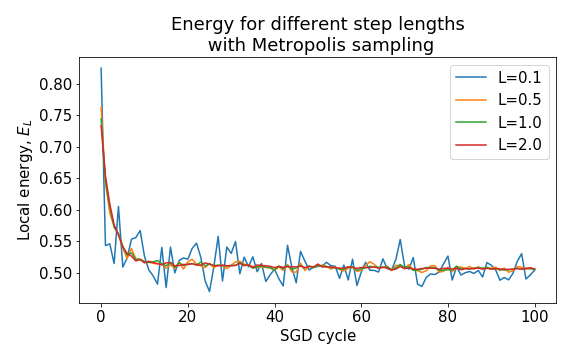
\includegraphics[width=0.7\linewidth, height=0.5\linewidth]{L_01_20.png}
	\caption{Local energy as function of the SGD cycle for various Metropolis step lengths. Here we see that for $L\geq0.5$ we get more or less stable curves, and they all reach an equilibrium around 20 SGD cycles. \label{fig:check_L}}
\end{figure} 

\begin{table}[htbp!]
	\centering
	\begin{tabular}{|c|c|c|c|c|c|}
		\hline \rule{0pt}{13pt}
		L & 0.01 & 0.1 & 0.5 & 1.0 & 2.0 \\
		\hline \rule{0pt}{13pt}
		A & 0.999 &  0.987 & 0.935 & 0.870 & 0.748 \\
		\hline
	\end{tabular}
	\caption{Table for the acceptance rate (A) of the Metropolis sampling for various step lengths (L). See here that the smaller the step length is, the bigger and better is the acceptance rate. \label{tab:Met_A}}
\end{table}

With the chosen step length $L=0.5$, we experiment with the learning rate to see how it affects the system. In Figure \ref{fig:check_learnrate_Met} we see how the local energy behaves as a function of the SGD cycles for various learning rates. For higher learning rates we see a faster convergence time. The change in learning rate does not affect the acceptance rate of the system. When $\eta=0.01$, the solution does not converge to the analytical solution within 100 SGD cycles like the others. When $\eta>0.6$, the solution simply diverges and is not included here. So we choose $\eta=0.2$ as the learning rate parameter, since the solution converges under 20 SGD cycles and does not converge too fast.

\begin{figure}[htbp!]
	\centering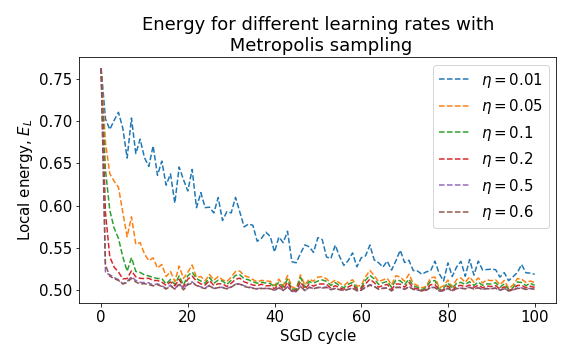
\includegraphics[width=0.7\linewidth, height=0.5\linewidth]{Met_learnrate.png}
	\caption{Local energy as function of the SGD cycle for various learning rates with the Metropolis sampling and $L=0.5$. See here that the higher the learning rate is, the faster the solution reaches the equilibrium for these selected values of learning rates. \label{fig:check_learnrate_Met}}
\end{figure} 

\subsubsection{Importance Sampling}
\label{subsubsect:Results_nonint_Importance}
Then we do the same analysis with the Importance sampling instead of Metropolis. The parameters we use are described in the Methods section \ref{subsubsect:Method_Nonint_Importance}. Now we have to find the best time step parameter $\Delta t$, which satisfies the same compromise as for $L$ in Metropolis. In Figure \ref{fig:check_dt} we see how the local energy as a function of the SGD cycles behaves for various time steps. The higher $\Delta t$ is, the better is the convergence towards the exact solution. For $\Delta t\geq 0.05$, we see that the convergence of the solution becomes quite good. So we want a $\Delta t\geq0.05$. Once again we look at the acceptance rate in Table \ref{tab:Imp_A} for the different time steps to find the best time step parameter for the sampling method. When $\Delta t>0.5$ the acceptance rate is not that good. When $\Delta t<0.1$ the acceptance rate is too close to zero, meaning that we accept more or less every move such that we do not move enough towards the minimum energy of the system. By looking at the acceptance rate, $\Delta t=0.5$ seems to be the best parameter, which fits well with our conclusion from Figure \ref{fig:check_dt}.

\begin{figure}[t!]
	\centering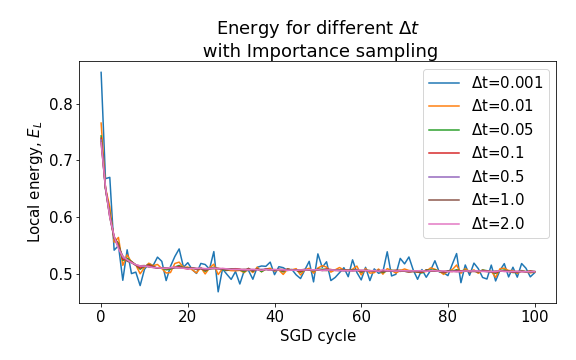
\includegraphics[width=0.7\linewidth, height=0.5\linewidth]{dt.png}
	\caption{Local energy as function of the SGD cycle for various Importance sampling time steps. For $\Delta t\geq0.05$ we get smooth curves and fast convergence for all parameters used. \label{fig:check_dt}}
\end{figure}

\begin{table}[htbp!]
	\centering
	\begin{tabular}{|c|c|c|c|c|c|c|c|}
		\hline \rule{0pt}{13pt}
		$\Delta t$ & 0.001 & 0.01 & 0.05 & 0.1 & 0.5 & 1.0 & 2.0 \\
		\hline \rule{0pt}{13pt}
		A & 0.999996 & 0.9998 & 0.998 & 0.994 & 0.93 & 0.81 & 0.56 \\
		\hline
	\end{tabular}
	\caption{Table for the acceptance rate (A) of the Importance sampling for various time step ($\Delta t$). See here that the smaller the time step is, the bigger and better is the acceptance rate. \label{tab:Imp_A}}
\end{table}

\newpage
With the chosen time step $\Delta t=0.5$, we experiment with the learning rate once again. In Figure \ref{fig:check_learnrate_Imp} we see how the local energy behaves for various learning rates. We see a similar behavior of the solution as we got with Metropolis in Figure \ref{fig:check_learnrate_Met}. The only difference seems to be that the curves with Importance sampling are much smoother than with Metropolis. Since they are so similar, we make the same conclusion for the best learning rate $\eta=0.2$.

\begin{figure}[htbp!]
	\centering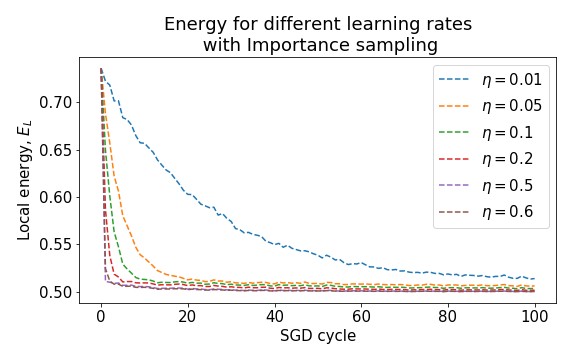
\includegraphics[width=0.7\linewidth, height=0.5\linewidth]{Imp_learnrate.png}
	\caption{Local energy as function of the SGD cycle for various learning rates with the Importance sampling and $\Delta t=0.5$. See here that the higher the learning rate is, the faster the solution reaches the equilibrium. Get very similar curves as for Metropolis, but in this case the curves are much smoother. \label{fig:check_learnrate_Imp}}
\end{figure} 

\subsubsection{Gibbs Sampling}
\label{subsubsect:Results_nonint_Gibbs}
The last sampling method we use is the Gibbs sampling. The parameters we use are described in the Methods section \ref{subsubsect:Method_Nonint_Gibbs}. For this sampling method we have to tune the $\sigma$ parameter which we used as $\sigma=1.0$ for the other two sampling methods. In Figure \ref{fig:check_sigma} we see how the local energy as a function of the SGD cycles behaves for various sigmas. From the figure we can clearly see that the Gibbs sampling converges towards different energies for different sigmas. So the Gibbs sampling is very dependent on which value we use for $\sigma$. Here we see that when we use $\sigma=0.6$ or 0.7, the solution converges towards the analytical ground state energy. $\sigma=0.6$ reach equilibrium in fewer SGD cycles than $\sigma=0.7$ does, which is why we might assume $\sigma=0.6$ as the best Gibbs parameter in this case. With this sampling method, the acceptance rate is always 1. So we get no new information by looking at the acceptance rate when choosing the best sigma parameter.

\begin{figure}[htbp!]
	\centering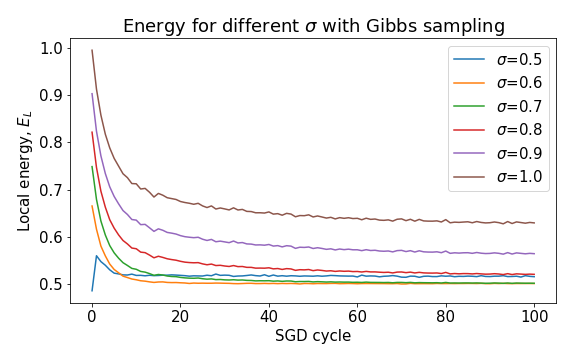
\includegraphics[width=0.7\linewidth, height=0.5\linewidth]{sigma.png}
	\caption{Local energy as function of the SGD cycle for various Gibbs sampling sigmas. For $\sigma=[0.6, 0.7]$ we see convergence towards the analytical ground state energy. \label{fig:check_sigma}}
\end{figure}

\newpage
With $\sigma=0.6$, we experiment with the learning rate. In Figure \ref{fig:check_learnrate_Gib} we see how the local energy behaves for various learning rates. The plots are similar to Importance sampling, except that for $\sigma\geq0.5$ the curves jump at the beginning before a fast convergence towards the exact solution. The best learning rate parameter seems to be $\eta=0.2$, as for the other sampling methods. 

In Figure \ref{fig:check_learnrates_Gib} we see a comparison of the local energy with the two best learning rates for both $\sigma=0.6$ and 0.7. There we see that $\eta=0.2$ is the best learning rate for both sigmas. For the smaller sigma, we reach equilibrium faster than for the bigger. From these figures we could conclude with that $\sigma=0.6$ would be the best parameter to use with Gibbs sampling. By further testing of the local energy with these sigmas, the final local energy seems to be best when we use $\sigma=0.7$. So even though $\sigma=0.6$ reaches equilibrium the fastest, it's $\sigma=0.7$ that gives the best final energy. That is why we use $\sigma=0.7$ as the best Gibbs sampling parameter.

\begin{figure}[htbp!]
	\centering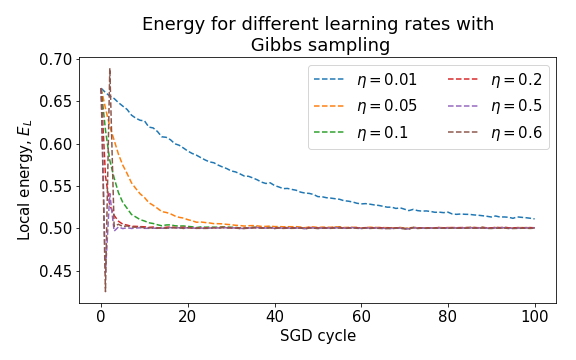
\includegraphics[width=0.75\linewidth, height=0.55\linewidth]{Gib_learnrate.png}
	\caption{Local energy as function of the SGD cycle for various learning rates with the Gibbs sampling and $\sigma=0.6$. See here that the higher the learning rate is, the faster the solution reaches the equilibrium. Get very similar curves as for Importance sampling, except for the two biggest parameters which deviates some in the beginning. \label{fig:check_learnrate_Gib}}
\end{figure} 

\begin{figure}[htbp!]
	\centering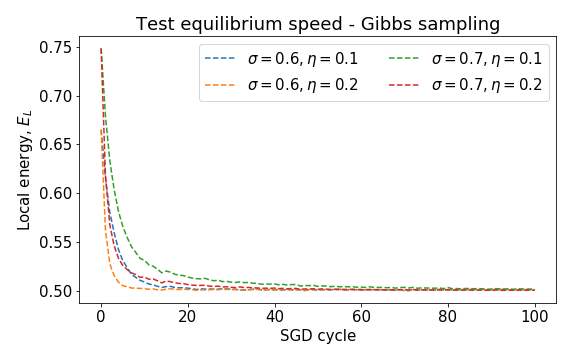
\includegraphics[width=0.75\linewidth, height=0.55\linewidth]{Gib_learnrate_test.png}
	\caption{Local energy as function of the SGD cycle for various learning rates with the Gibbs sampling and $\sigma=0.6$ and $\sigma=0.7$. Further check for the best sigma  and learning rate parameters. \label{fig:check_learnrates_Gib}}
\end{figure} 

\newpage
\subsubsection{Local Energy Analysis of Sampling Methods}
\label{subsubsect:Results_nonint_Analysis}
With all the best parameters for the three sampling methods, we will look at the final energies produced from each sampling method when we vary the number of particles ($N_P$), dimensions ($D$) and hidden nodes ($N_H$). In Table \ref{tab:Nonint_energies} we see the local energies for non-interacting electrons produced by each sampling method as described in the caption of the table. To produce these local energies we use $N_{SGD}=150$ and $\eta=0.2$ for all three sampling methods. The Metropolis step length is $L=0.5$, and the Importance time step is $\Delta t=0.5$. With these two sampling methods we also use $\sigma=1.0$, while we use $\sigma=0.7$ with Gibbs sampling.

The most accurate sampling method seems to be Gibbs, since the produced local energies are on average more close to the analytical ground state energies in terms of both accuracy and the errors (from blocking). In the case of CPU time for doing the computation, the Metropolis is the fastest sampling method while Importance sampling gave the slowest CPU time. For all three sampling methods we see that the local energies for $N_P=1,D=2$ and $N_P=2,D=1$ are the same for each sampling method respectively. From this it seems that the computation of the energy is the same when the sum of the number of particles and dimensions are the same with that sampling method.

Another thing we notice when we increase the number of hidden nodes but keep $N_P$ and $D$ the same, is that the average $E_L$ with blocking increases by a small amount each time $N_H$ is increased. On average, the errors also increase as the number of hidden nodes as increased. This also goes for the time to do the full MC calculation for each sampling method. 

\begin{table}[htbp!]
	\centering
	%\hspace{-1.0cm}
	\begin{tabular}{ |c|c|c|c|c|c|c| }
		\hline \rule{0pt}{13pt}
		$N_P$ & D & $N_H$ & $E_A$ & $E_L^M$ & $E_L^I$ & $E_L^G$ \\
		\hline \rule{0pt}{13pt}%
		1 & 1 & 1 & 0.5 & 0.500$\pm1.6\cdot10^{-8}$ & 0.500$\pm3.6\cdot10^{-9}$ & 0.500$\pm1.4\cdot10^{-5}$ \\
		%\hline \rule{0pt}{13pt}
		1 & 1 & 2 & 0.5 & 0.501$\pm5.0\cdot10^{-4}$ & 0.501$\pm6.0\cdot10^{-5}$ & 0.500$\pm2.3\cdot10^{-5}$ \\
		\hline \rule{0pt}{13pt}%
		1 & 2 & 1 & 1.0 & 1.050$\pm3.5\cdot10^{-3}$ & 1.001$\pm8.1\cdot10^{-5}$ & 1.000$\pm2.6\cdot10^{-5}$ \\
		%\hline \rule{0pt}{13pt}
		1 & 2 & 2 & 1.0 & 1.002$\pm5.6\cdot10^{-4}$ & 1.001$\pm1.1\cdot10^{-4}$ & 1.000$\pm2.9\cdot10^{-5}$ \\
		\hline \rule{0pt}{13pt}%
		2 & 1 & 1 & 1.0 & 1.050$\pm3.5\cdot10^{-3}$ & 1.001$\pm8.1\cdot10^{-5}$ & 1.000$\pm2.6\cdot10^{-5}$ \\
		%\hline \rule{0pt}{13pt}
		2 & 1 & 2 & 1.0 & 1.002$\pm5.6\cdot10^{-4}$ & 1.001$\pm1.1\cdot10^{-4}$ & 1.000$\pm2.9\cdot10^{-5}$ \\
		\hline \rule{0pt}{13pt}%
		2 & 2 & 1 & 2.0 & 1.999$\pm3.0\cdot10^{-4}$ & 2.000$\pm6.4\cdot10^{-5}$ & 2.000$\pm3.0\cdot10^{-5}$ \\
		%\hline \rule{0pt}{13pt}
		2 & 2 & 2 & 2.0 & 2.000$\pm5.1\cdot10^{-4}$ & 2.001$\pm1.1\cdot10^{-4}$ & 2.000$\pm2.7\cdot10^{-5}$ \\
		%\hline \rule{0pt}{13pt}
		2 & 2 & 3 & 2.0 & 2.002$\pm8.5\cdot10^{-4}$ & 2.002$\pm1.7\cdot10^{-4}$ & 2.000$\pm3.4\cdot10^{-5}$ \\
		%\hline \rule{0pt}{13pt}
		2 & 2 & 4 & 2.0 & 2.001$\pm9.3\cdot10^{-4}$ & 2.002$\pm2.0\cdot10^{-4}$ & 2.000$\pm3.5\cdot10^{-5}$ \\
		\hline
	\end{tabular}	
	\caption{Table for the final local energy (in a.u.) of non-interacting electrons with the three sampling methods Metropolis ($E_L^M$), Importance ($E_L^I$) and Gibbs ($E_L^G$) with blocking errors, and the analytical ground state energy ($E_A$). \label{tab:Nonint_energies}}
\end{table}

\subsection{Interacting Electrons}
\label{subsect:Results_int}
With interaction between the electrons, we will do the same analysis of the system as we did for non-interacting electrons. The difference is that we now only look at two electrons in 2D since Pauli's principle is not accounted for. In this case we expect the analytical ground state energy to be 3 a.u (sect. \ref{subsubsect:Analytical E_L}). The numerical parameters we use are described in the Methods section \ref{subsect:Method_int}.

\subsubsection{Metropolis Sampling}
\label{subsubsect:Results_int_Metropolis}
We use the same step length $L=0.5$ that we found in the non-interacting case for Metropolis sampling first. Then we once again will experiment with the learning rate of this interacting system. In Figure \ref{fig:check_learnrate_Int_Met} we see how the local energy behaves for various learning rates. Here we see that as the learning rate increase, the faster the solution converges to equilibrium. Since there is such a big spread of data points for the local energy, it is not easy to see what the solution converges towards exactly. This can be fixed by doing a linear regression fit of the data points. By doing a linear regression on the data points after equilibrium for each learning rate respectively, we get that they do not converge exact to the exact ground state energy. The computed energies after linear regression gives the converged energies around 3.08 a.u., which is a little higher than the exact energy of 3 a.u. From this figure we can conclude that $\eta=0.2$ seems to give the best solution like for non-interacting Metropolis.

The interacting solution uses more SGD cycles to reach equilibrium than the non-interacting system. So the system needs more cycles to adapt to the interacting wave function than for a non-interacting wave function. The non-interacting Metropolis only needed around 20 SGD cycles to reach equilibrium, while the best case here needs around 250-300 SGD cycles to reach equilibrium.

\begin{figure}[ht!]
	\centering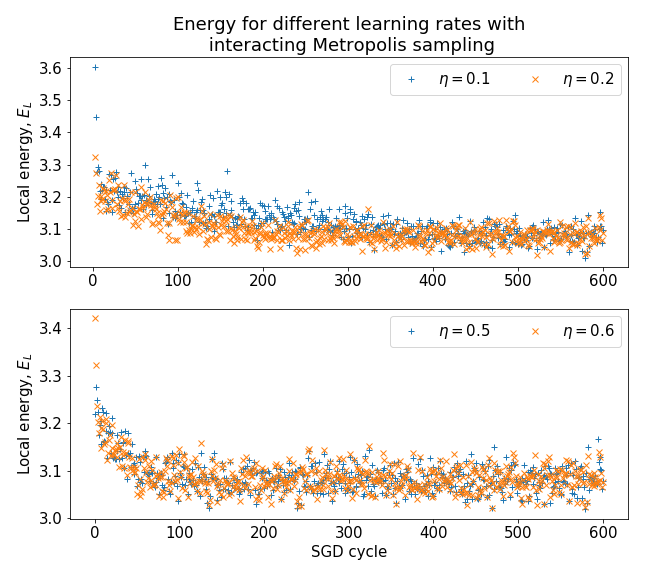
\includegraphics[width=0.8\linewidth, height=0.8\linewidth]{Int_Met_learnrate.png}
	\caption{Local energy as function of the SGD cycle for various learning rates with the Metropolis sampling and $L=0.5$ for two interacting electrons in 2D. The higher the learning rate is, the faster the solution converges. The energy curves are much thicker compared to non-interacting electrons in Figure \ref{fig:check_learnrate_Met}. \label{fig:check_learnrate_Int_Met}}
\end{figure} 

\newpage
Changing the number of hidden nodes did not change much for the non-interacting system. We test now the interacting system in terms of the number of hidden nodes to see if we get any differences. In Figure 
\ref{fig:check_hidden_Int_Met} we see the local energy when we use up till four hidden nodes in our neural network. Using one hidden node gives a much higher energy after equilibrium than the other three cases. It looks like when using a higher number of hidden nodes, the system manages to reach equilibrium in fewer SGD cycles. With three and four hidden nodes we get very similar behavior of the energy solutions, but we can barely see that four nodes drops the solution a little bit faster.

\begin{figure}[t!]
	\centering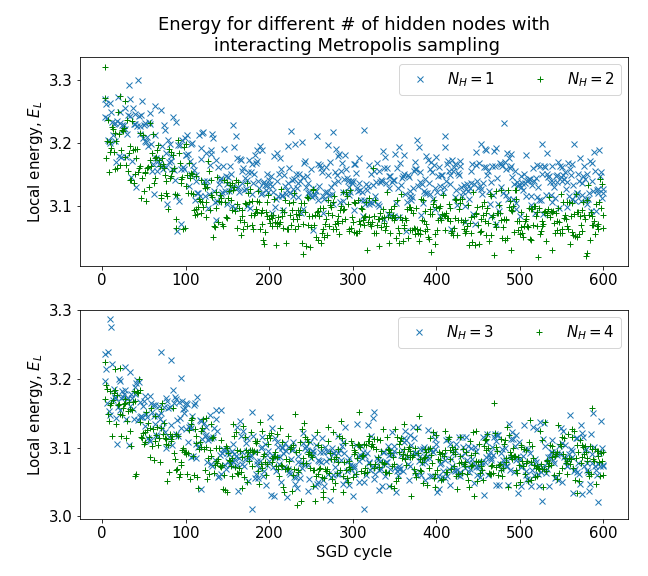
\includegraphics[width=0.8\linewidth, height=0.8\linewidth]{Hidden_Int_Met.png}
	\caption{Local energy as function of the SGD cycle for various number of hidden nodes with the Metropolis sampling, $L=0.5$ and $\eta=0.2$ for two interacting electrons in 2D. Using one hidden node does not give as good solution as the two, three and four hidden nodes. \label{fig:check_hidden_Int_Met}}
\end{figure} 

\newpage
\subsubsection{Importance Sampling}
\label{subsubsect:Results_int_Importance}
In the non-interacting case with Importance sampling when varying the learning rate, we got a much smaller spread of data points/smoother curve compared to Metropolis sampling. This is also the case in the interacting system with Importance sampling. By looking at Figure \ref{fig:check_learnrate_Int_Imp} we see that the spread of data points/thickness of the curve is smaller/thinner than for interacting Metropolis. The form of the curves are the same for both cases, where a higher learning rate gives faster equilibrium convergence. For $\eta=0.1$, the solution takes a lot of SGD cycles before reaching equilibrium compared to the other learning rates. We use the same conclusion like before for why we choose the same learning rate $\eta=0.2$ here as well.

\begin{figure}[t!]
	\centering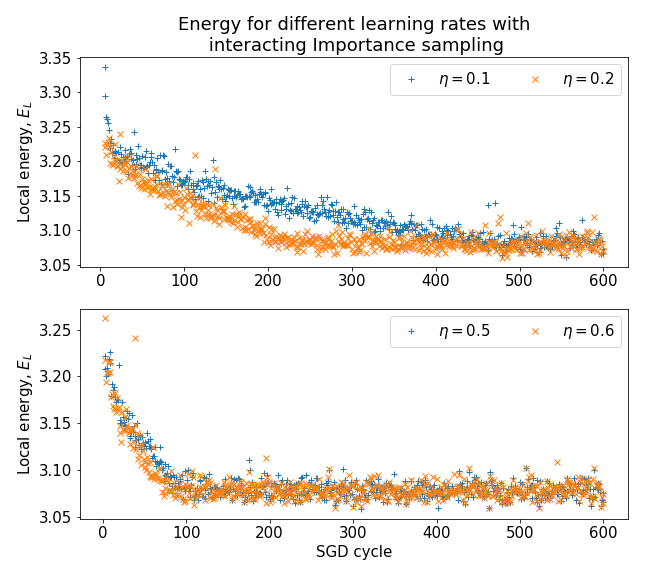
\includegraphics[width=0.8\linewidth, height=0.8\linewidth]{Int_Imp_learnrate.png}
	\caption{Local energy as function of the SGD cycle for various learning rates with the Importance sampling and $\Delta t=0.5$ for two interacting electrons in 2D. The higher the learning rate is, the faster the solution converges. The energy curves are much thinner compared to interacting Metropolis in Figure \ref{fig:check_learnrate_Int_Met}. \label{fig:check_learnrate_Int_Imp}}
\end{figure}

\newpage
In Figure \ref{fig:check_hidden_Int_Imp} we vary the number of hidden nodes with Importance sampling. As with the learning rate, the spread of data points are much smaller for Importance than for Metropolis. Now we more clearly see that as the number of hidden nodes increases, the quicker in terms of SGD cycles the solution reaches its equilibrium. Still they converge to more or less the same local energy. Again, only using one hidden node converges to a higher energy than for two, three and four hidden nodes which seem to converge to around energy of 3.08 a.u.

\begin{figure}[t!]
	\centering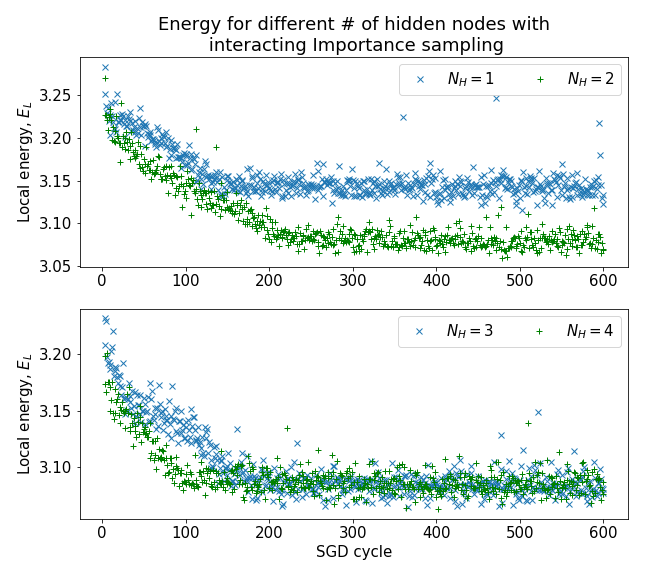
\includegraphics[width=0.8\linewidth, height=0.8\linewidth]{Hidden_Int_Imp.png}
	\caption{Local energy as function of the SGD cycle for various number of hidden nodes with the Importance sampling, $\Delta t=0.5$ and $\eta=0.2$ for two interacting electrons in 2D. Using one hidden node does not give as good solution as using two, three and four hidden nodes. \label{fig:check_hidden_Int_Imp}}
\end{figure} 

\newpage
\subsubsection{Gibbs Sampling}
\label{subsubsect:Results_int_Gibbs}
As with the non-interacting case, we use the same Gibbs parameter $\sigma=0.7$. With this parameter we test the learning rate with Gibbs sampling. In Figure \ref{fig:check_learnrate_Int_Gib} we see that the local energy drops quicker towards equilibrium than the other sampling methods, before it oscillates a little around the equilibrium energy. The local energy which the solutions converge towards wit Gibbs sampling, are clearly a little closer to the analytical ground state energy than the other two sampling methods when we vary the learning rate. Like the other cases, a higher learning rate gives faster equilibrium where $\eta=0.1$ uses a lot more SGC cycles to reach equilibrium than the others. The two highest learning rates are close to each other like earlier. The best learning rate seems to be $\eta=0.2$, like before.

\begin{figure}[t!]
	\centering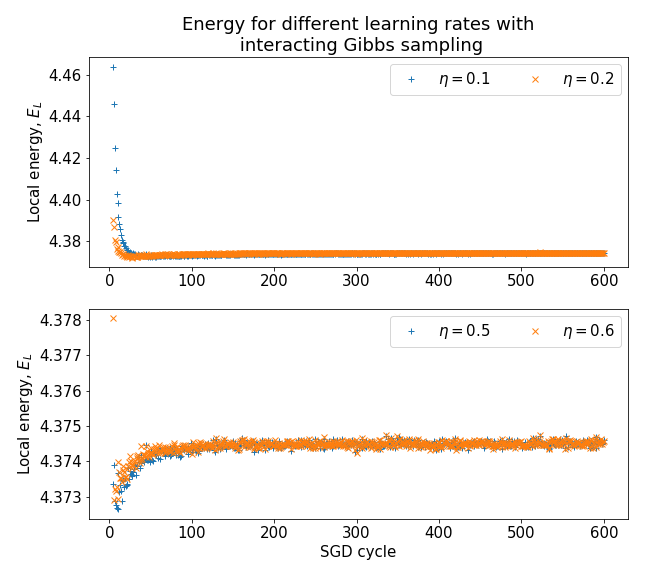
\includegraphics[width=0.8\linewidth, height=0.8\linewidth]{Int_Gib_learnrate.png}
	\caption{Local energy as function of the SGD cycle for various learning rates with the Gibbs sampling and $\sigma=0.7$ for two interacting electrons in 2D. The higher the learning rate is, the faster the solution converges towards equilibrium energy. \label{fig:check_learnrate_Int_Gib}}
\end{figure}

\newpage
In Figure \ref{fig:check_hidden_Int_Gib} we vary the number of hidden nodes using the best learning rate with Gibbs sampling. Like for Metropolis and Importance, using one hidden node gives a much higher local energy. With two, three and four hidden nodes we get convergence towards a local energy of around 3.05-3.06 a.u. Once again, using more hidden nodes in our NN leads to a faster convergence towards equilibrium. After around 250 SGD cycles we see that all solutions seem to have reached equilibrium energy.

\begin{figure}[t!]
	\centering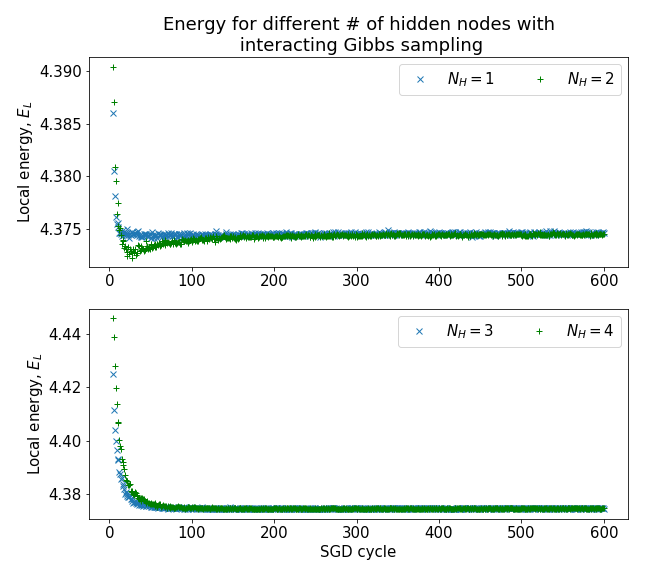
\includegraphics[width=0.8\linewidth, height=0.8\linewidth]{Hidden_Int_Gib.png}
	\caption{Local energy as function of the SGD cycle for various number of hidden nodes with the Gibbs sampling, $\sigma=0.7$ and $\eta=0.2$ for two interacting electrons in 2D. Using more than one hidden node seem to give good convergence towards equilibrium. \label{fig:check_hidden_Int_Gib}}
\end{figure}

\newpage
\subsubsection{Local Energy Analysis of Sampling Methods}
\label{subsubsect:Results_int_Analysis}
With the best parameters for the three sampling methods, we look more at how the computed local energies are as we vary the number of hidden nodes. The final local energies for two interacting electrons in 2D can be seen in Table \ref{tab:Int_energies}. The blocking method is applied on the produced energy data with a linear regression fit after equilibrium. Here we have used $N_{SGD}=600$ and $\eta=0.2$ for all the sampling methods, and used the same best sampling parameters as in the non-interacting cases.

In the non-interacting case we got that the Gibbs sampling gave the best solutions. We would also expect this in the interacting case since the sampling method should not change the solution of the model that significantly, this is also the case with interaction in our system. In this case the standard Metropolis gives slightly better average energies than Importance. The Gibbs method is clearly the best sampling method, which we see by looking at the computed local average energies in the table for various hidden nodes. The best average energies for each sampling method is when we use two hidden nodes.

Like with the non-interacting system, the Metropolis is the fastest method and Importance is the slowest method of the three regarding CPU time. Also here, the CPU time for doing the energy computations increase when we use a higher number of hidden nodes. Using one hidden node gives the fastest CPU time, but gives a higher final energy for all sampling methods.

\begin{table}[htbp!]
	\centering
	%\hspace{-1.0cm}
	\begin{tabular}{ |c|c|c|c|c|c|c| }
		\hline \rule{0pt}{14pt}
		$N_P$ & D & $N_H$ & $E_A$ & $E_L^M$ & $E_L^I$ & $E_L^G$ \\
		\hline \rule{0pt}{13pt}%
		2 & 2 & 1 & 3.0 & 3.140$\pm1.3\cdot10^{-5}$ & 3.144$\pm4.0\cdot10^{-5}$ & 3.131$\pm5.3\cdot10^{-5}$ \\
		%\hline \rule{0pt}{13pt}
		2 & 2 & 2 & 3.0 & 3.081$\pm7.7\cdot10^{-5}$ & 3.081$\pm1.2\cdot10^{-4}$ & 3.062$\pm5.2\cdot10^{-5}$ \\
		%\hline \rule{0pt}{13pt}
		2 & 2 & 3 & 3.0 & 3.082$\pm1.9\cdot10^{-4}$ & 3.084$\pm3.3\cdot10^{-5}$ & 3.066$\pm2.8\cdot10^{-4}$ \\
		%\hline \rule{0pt}{13pt}
		2 & 2 & 4 & 3.0 & 3.084$\pm8.7\cdot10^{-5}$ & 3.086$\pm3.5\cdot10^{-5}$ & 3.067$\pm4.2\cdot10^{-5}$ \\
		\hline
	\end{tabular}	
	\caption{Table for the final local energy of interacting electrons with the three sampling methods Metropolis ($E_L^M$), Importance ($E_L^I$) and Gibbs ($E_L^G$) with blocking errors, and the analytical ground state energy ($E_A$). The Gibbs sampling method provides the best average energies. \label{tab:Int_energies}}
\end{table}


\section{Conclusion}
\label{sect:Conclusion}
In this project we have used a restricted Boltzmann machine and neural network with a variational Monte Carlo method to compute the ground state energy of interacting and non-interacting systems consisting of electrons in a 2D isotropic harmonic oscillator potential. These ground state energies have been computed both analytically and numerically to check how well the RBM neural network can reproduce the energy of the system. To do this we have used the standard brute-force Metropolis sampling, Importance sampling and Gibbs sampling methods. To optimize the system we also used a stochastic gradient descent method with a constant learning rate, and used blocking for a statistical analysis of the energy errors. With these methods we looked at different choices of parameters for each sampling method to see how they affected our computation of the ground state energies.

In the non-interacting case we got energies very close to the analytically calculated ground state energies for all the three sampling methods. Here the Gibbs sampling gave the best solutions with the smallest errors. The Metropolis method was the fastest method in CPU time, but it also gave slightly worse solutions than the other two sampling methods.

For the interacting case we got energies a little higher than the analytically calculated energies. For all three sampling methods, we got reasonably good energies close to the analytical energies. The Metropolis was also the fastest method in CPU time here, and gave energies a little better than the Importance method, which where the slowest method again. As for non-interacting electrons, the Gibbs sampling method gave the best local energies closest to the analytical ground state energies. 

From our analysis in this project, we can conclude that the Gibbs sampling method seems to be the best sampling method for this RBM NN system with electrons.

For future work, we could try to use other optimization methods like ADAM. We could also do a steepest descent method on some of the parameters we have used to make them adapt to make a better fit to the evolving behavior of the system. To get faster CPU times we could implement parallelization by using MPI. The system we have looked at in this project did not include Pauli's principle. So this is also something we could implement in future work, and eventually extend our system with more particles with higher dimensions.

\appendix
\section*{Appendix:}
\section{Kinetic Energy Derivation}
\label{appendix:E_k}
Here we will derive the kinetic energy part of the local energy expression in equation \ref{eq:EL_kin_pot_int}. We start by rewriting the kinetic part:
\begin{equation}
\label{eq:Wave_Laplacian}
\frac{1}{\Psi}\nabla^2\Psi=\nabla^2\ln\Psi + (\nabla\ln\Psi)^2
\end{equation}
Then we find the logarithm of the wave function:
\begin{equation}
\ln\Psi=-\sum_{i=1}^{M}\frac{(X_i-a_i)^2}{2\sigma^2}+\sum_{j}^{N}\ln\left(1+e^{b_j + \sum_{i}^{M}\frac{X_iw_{ij}}{\sigma^2}}
\right)
\end{equation}
Than we take the gradient with respect to $X_k$:
\begin{align}
\label{eq:Gradient_Xk}
\frac{\partial }{\partial X_k}\ln\Psi&=-\frac{X_k-a_k}{\sigma^2} + \sum_{j}^{N}\frac{e^{b_j + \sum_{i}^{M}\frac{X_iw_{ij}}{\sigma^2}}}{1+e^{b_j + \sum_{i}^{M}\frac{X_iw_{ij}}{\sigma^2}}}\cdot\frac{w_{kj}}{\sigma^2}\nonumber\\ &=-\frac{X_k-a_k}{\sigma^2} + \sum_{j}^{N}\frac{1}{1+e^{-b_j - \sum_{i}^{M}\frac{X_iw_{ij}}{\sigma^2}}}\cdot\frac{w_{kj}}{\sigma^2}\nonumber\\
&=-\frac{X_k-a_k}{\sigma^2} + \sum_{j}^{N}\Sigma(u_j)\cdot\frac{w_{kj}}{\sigma^2}
\end{align}
The denominator in the fraction above has a famous name called the logistic sigmoid function. For simplicity we will use $\Sigma$ for the sigmoid function as
\begin{equation}
\label{eq:sigmoid}
\Sigma(u_j)=\frac{1}{1+e^{u_j}}\quad \text{with} \quad u_j=-b_j - \sum_{i}^{M}\frac{X_iw_{ij}}{\sigma^2}.
\end{equation}
The second derivative is then:
\begin{align}
\label{eq:2nd_Gradient_Xk}
\frac{\partial^2 }{\partial X_k^2}\ln\Psi&=-\frac{1}{\sigma^2}+\sum_{j}^{N}\Sigma(u_j)\cdot\Sigma(-u_j)\cdot\frac{w_{kj}^2}{\sigma^4}
\end{align}
The full kinetic energy part in equation \ref{eq:Wave_Laplacian} is then:
\begin{align*}
\frac{1}{\Psi}\nabla^2\Psi&= -\frac{M}{\sigma^2} +\sum_{i}^{M}\sum_{j}^{N}\Sigma(u_j)\cdot\Sigma(-u_j)\cdot\frac{w_{ij}^2}{\sigma^4} +\sum_{i}^{M}\frac{X_i-a_i}{\sigma^2}\\ 
&\quad -2\sum_{i}^{M}\frac{X_i-a_i}{\sigma^2}\sum_{j}^{N}\Sigma(u_j)\cdot\frac{w_{ij}}{\sigma^2} 
+\sum_{i}^{M}\sum_{j}^{N}(\Sigma(u_j))^2\cdot\frac{w_{ij}^2}{\sigma^4}
\end{align*}

\section{Gibbs Kinetic Energy Derivation}
\label{appendix:Gibbs_Ek}
With the new representation of the wave function as $\Psi_G(\textbf{X})=\sqrt{F_{rbm}(\textbf{X})}$, we get that $\ln(\Psi_G)=\frac{1}{2}\ln(\Psi)$. This means that the kinetic energy part of the local energy becomes:
\begin{align*}
\frac{1}{\Psi_G}\nabla^2\Psi_G&=\nabla^2\ln\Psi_G + (\nabla\ln\Psi_G)^2 =\frac{1}{2}\nabla^2\ln\Psi + \frac{1}{4}(\nabla\ln\Psi)^2\\
&=-\frac{M}{2\sigma^2} +\frac{1}{2}\sum_{i}^{M}\sum_{j}^{N}\Sigma(u_j)\cdot\Sigma(-u_j)\cdot\frac{w_{ij}^2}{\sigma^4} +\frac{1}{4}\sum_{i}^{M}\frac{X_i-a_i}{\sigma^2}\\ 
&\quad -\frac{1}{2}\sum_{i}^{M}\frac{X_i-a_i}{\sigma^2}\sum_{j}^{N}\Sigma(u_j)\cdot\frac{w_{ij}}{\sigma^2} 
+\frac{1}{4}\sum_{i}^{M}\sum_{j}^{N}(\Sigma(u_j))^2\cdot\frac{w_{ij}^2}{\sigma^4}
\end{align*}

\section{Analytic Derivation of the Local Energy}
\label{appendix:Analytic_EL}
\underline{* 1 particle in 1D:}\\
To derive the analytic expressions for the local energies we use the harmonic oscillator wave function in equation \ref{eq:simple_wf}. For the simplest case with one particle in 1D, the eigenvalues ($\epsilon$) of the Hamiltonian are dependent on the principal quantum number $n_x$ in natural units as
\begin{equation*}
\epsilon_{n_x}=\omega(n_x+\frac{1}{2}).
\end{equation*}
The local energy then becomes;
\begin{equation*}
E_{n_x}=\frac{1}{\phi_{n_x}}H\phi_{n_x}=\epsilon_{n_x}=\omega(n_x+\frac{1}{2})
\end{equation*}
In the lowest-lying state $n_x=0 \quad \Rightarrow \quad E_0=\frac{\omega}{2}$.
\\ \\
\underline{* 1 particle in 2D:}\\
For one particle in 2D we get
\begin{align*}
H\phi_{n_x,n_y}=H\phi_{n_x}\cdot\phi_{n_y}+H\phi_{n_y}\cdot\phi_{n_x}= \epsilon_{n_x}\phi_{n_x,n_y}+\epsilon_{n_y}\phi_{n_x,n_y}.
\end{align*}
The local energy simply becomes:
\begin{equation*}
E_{n_x,n_y}=\frac{1}{\phi_{n_x,n_y}}H\phi_{n_x,n_y}=\epsilon_{n_x}+\epsilon_{n_y}=\omega(n_x+n_y+1)
\end{equation*}
In the lowest-lying state $n_x=n_y=0\quad \Rightarrow \quad E_{00}=\omega$.
\\ \\
\underline{* 2 particles in 2D:}\\
For two electrons in 2D, the wave function can be split into two single particle wave function parts:
\begin{align*}
\phi(\textbf{r}_1, \textbf{r}_2)=\phi_1(\textbf{r}_1)\cdot\phi_2(\textbf{r}_2)=\phi_{1 n_{x_1}, n_{y_1}}\cdot\phi_{2 n_{x_2}, n_{y_2}}\\
\rightarrow H\phi(\textbf{r}_1, \textbf{r}_2)=H\phi_1\cdot\phi_2+H\phi_2\cdot\phi_1=\epsilon_{n_{x_1},n_{y_1}}\phi_{1,2}+\epsilon_{n_{x_2},n_{y_2}}\phi_{1,2}
\end{align*}
The local energy becomes:
\begin{equation*}
E_{n_x,n_y}=\frac{1}{\phi(\textbf{r}_1, \textbf{r}_2)}H\phi(\textbf{r}_1, \textbf{r}_2)=\epsilon_{n_{x_1},n_{y_1}}+\epsilon_{n_{x_2},n_{y_2}}=\omega(n_{x_1}+n_{x_2}+n_{y_1}+ n_{y_2}+2)
\end{equation*}
In the lowest-lying state $n_{x_1}=n_{x_2}=n_{y_1}=n_{y_2}=0\quad \Rightarrow \quad E_{00}=2\omega$.\\

\section{Quantum Force Derivation}
\label{appendix:Quantum_force}
For the Importance sampling we need to derive the quantum force in equation \ref{eq:Quantum_force} analytically. Start be rewriting:
\begin{equation*}
\frac{\nabla\Psi_T}{\Psi_T}=\nabla_k\ln\Psi_T
\end{equation*}
This gradient we have already calculated in Appendix \ref{appendix:E_k}. This gives the quantum force as:
\begin{equation}
\label{eq:Quantum_force_derived}
F_k=-2\frac{X_k-a_k}{\sigma^2} + 2\sum_{j}^{N}\Sigma(u_j)\cdot\frac{w_{kj}}{\sigma^2}
\end{equation}
The quantum force is only used in Importance sampling, but can be altered for other wave functions (like the one in Gibbs sampling) as well.

\bibliographystyle{plainnat}
\bibliography{myrefs}
\end{document}